\documentclass[tikz,border=2pt]{standalone}
\usepackage{amsmath}
\usepackage{pgfplots}
\pgfplotsset{compat=1.18}
\usetikzlibrary{arrows.meta}
\begin{document}
% h(x)=1-x1*x2 on the open quadrant (quasi-convex, not convex); V={x1*x2>=1}. At p=(1,1) the gradient
% grad h(p)=(-1,-1) points out of V and is the normal of the supporting line x1+x2=2.
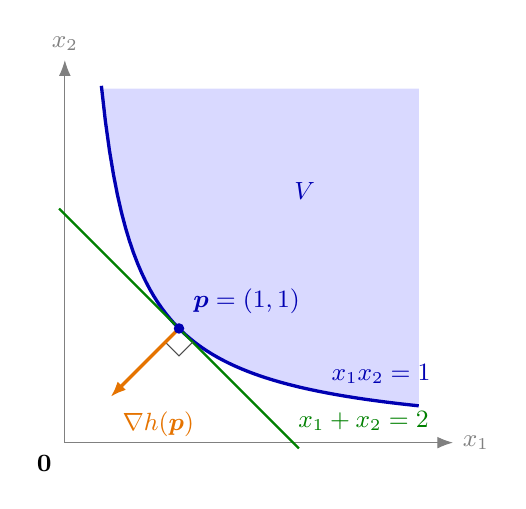
\begin{tikzpicture}[font=\small, >={Latex[length=2mm]}, x=1.45cm, y=1.45cm]
  \fill[blue!15] plot[domain=0.32:3.1, samples=80] (\x,{1/\x}) -- (3.1,3.1) -- (0.32,3.1) -- cycle;
  \draw[gray, ->] (0,0) -- (3.4,0) node[anchor=west] {$x_1$};
  \draw[gray, ->] (0,0) -- (0,3.35) node[anchor=south] {$x_2$};
  \draw[blue!70!black, very thick] plot[domain=0.32:3.1, samples=80] (\x,{1/\x});
  \node[blue!70!black, anchor=west] at (2.25,0.6) {$x_1x_2=1$};
  \node[blue!70!black] at (2.1,2.2) {$V$};
  \draw[green!50!black, thick] (-0.05,2.05) -- (2.05,-0.05);
  \node[green!50!black, anchor=south west] at (1.96,0.02) {$x_1+x_2=2$};
  % right-angle mark
  \draw[gray!60!black] (1.12,0.88) -- (1.0,0.76) -- (0.88,0.88);
  \draw[orange!90!black, very thick, ->] (1,1) -- (0.4,0.4);
  \node[orange!90!black, anchor=north west] at (0.42,0.36) {$\nabla h(\boldsymbol{p})$};
  \fill[blue!70!black] (1,1) circle (1.9pt);
  \node[blue!70!black, anchor=south west] at (1.04,1.04) {$\boldsymbol{p}=(1,1)$};
  \node[anchor=north east] at (-0.03,-0.03) {$\boldsymbol{0}$};
\end{tikzpicture}
\end{document}
